\subsection{Acciones desde el Interfaz Gráfico}
Siguiendo las directrices y conceptos de diseño de la interacción que se han 
repasado y señalado como importantes en las anteriores secciones, cabe ahora 
destacar las principales acciones a realizar en el demostrador público 
del sistema \gls{MOLDEAS}.

\begin{enumerate}
 \item Pantalla inicial del sistema MOLDEAS, ver Figura~\ref{fig:moldeas-web-screen} en el cual el usuario puede 
seleccionar y completar las variables de información de su perfil 
de búsqueda para la recuperación de información. La metáfora utilizada 
se basa en una simulación del tradicional ``carrito de la compra'' en la que 
el usuario puede seleccionar distintos códigos \gls{CPV}, \gls{NUTS}, establecer 
los rangos para algunas variables, etc. Se ha intentado simplificar 
al máximo este interfaz para evitar que una simple búsqueda se convierta 
en una tarea tediosa de rellenar un amplio formulario.

\begin{figure}[!htb]
\centering
	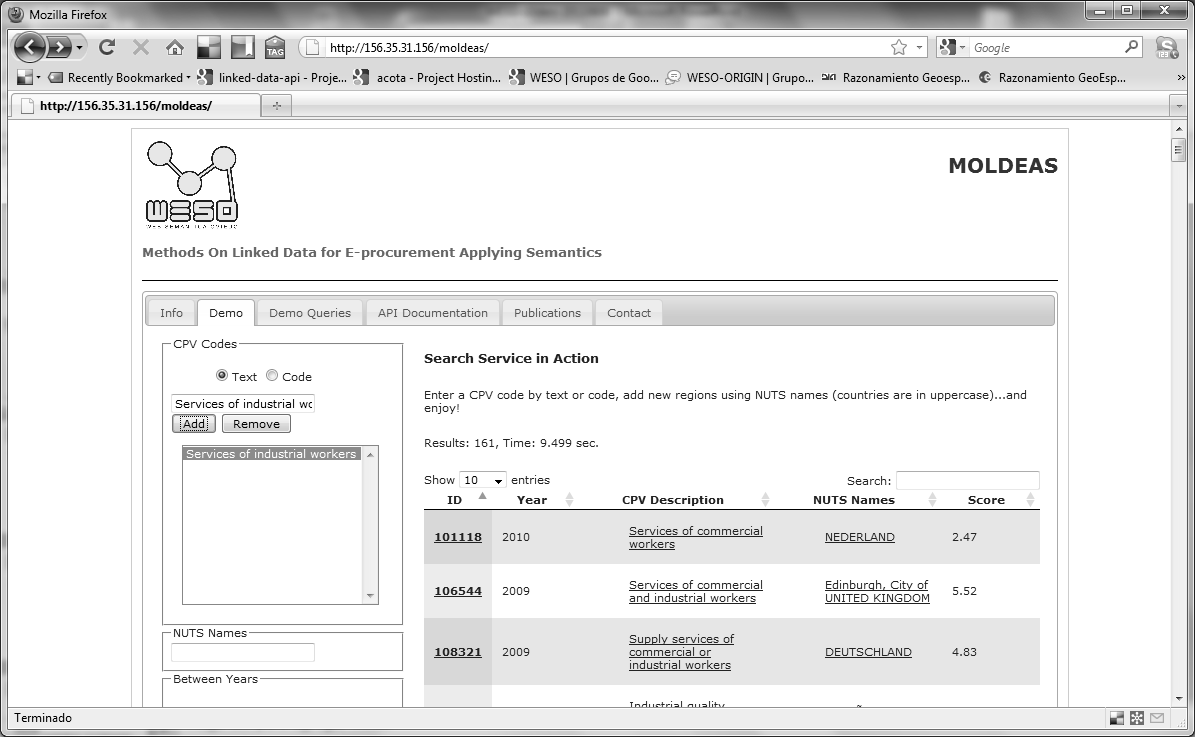
\includegraphics[width=14cm]{images/phd/moldeas/moldeas-web}
\caption{Ejemplo de pantalla inicial en \texttt{moldeas-web}.}
\label{fig:moldeas-web-screen}
\end{figure}


\item Una vez que el usuario ha seleccionado su perfil de búsqueda se ejecuta 
el proceso de recuperación de información presentando los resultados en forma 
tabular y mediante el uso de Exhibit, ver Figura~\ref{fig:moldeas-results-screen}. El usuario 
puede modificar su perfil de búsqueda y las consultas se lanzarán automáticamente una 
vez se detecten cambios. De la misma forma, el usuario puede filtrar los resultados, 
ordenarlos por relevancia, por sector, etc. e incluso visualizar la región en la 
que se han publicado los anuncios de licitación. La idea subyacente a esta 
interacción reside en que el usuario disponga del completo control de la presentación 
de los resultados obtenidos.


\begin{figure}[!htb]
\centering
	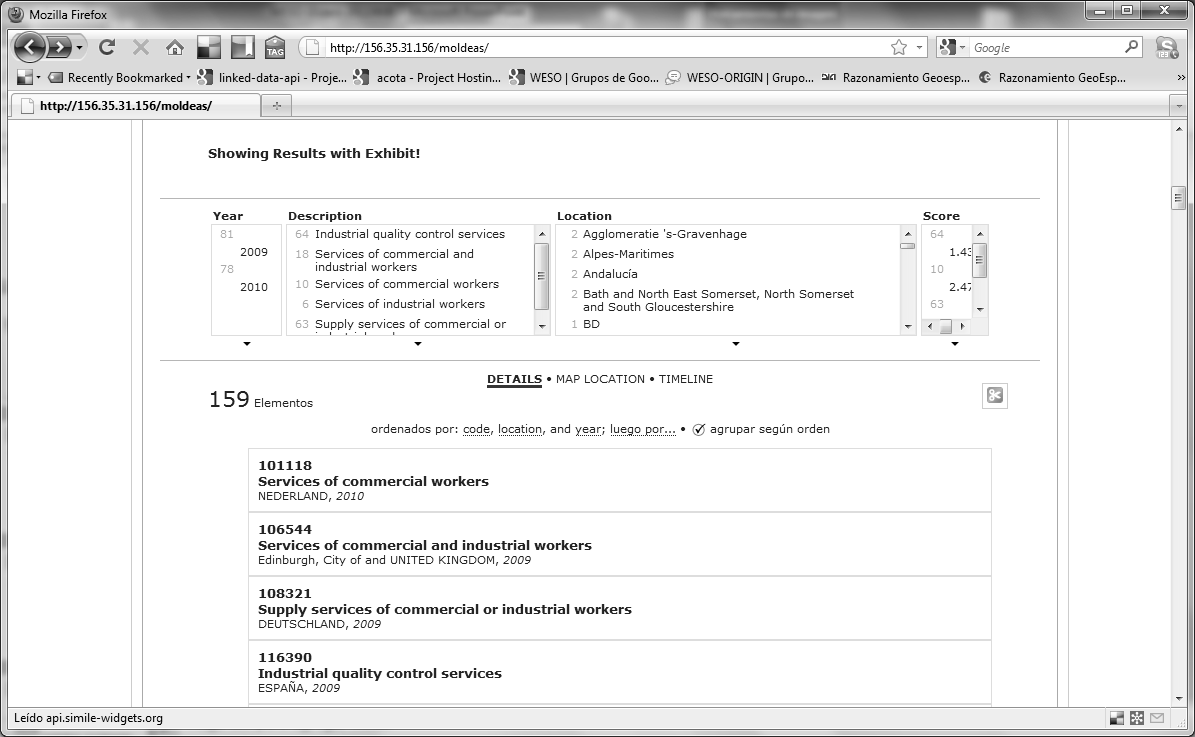
\includegraphics[width=14cm]{images/phd/moldeas/moldeas-results}
\caption{Ejemplo de pantalla de resultados en \texttt{moldeas-web}.}
\label{fig:moldeas-results-screen}
\end{figure}


\item En los resultados de búsqueda todas las \gls{URI}s presentadas son referenciables siguiendo 
las buenas prácticas de \linkeddata que han guiado la promoción de los datos a esta iniciativa. 
Es por ello que los datos propios del \dataset \gls{RDF} se pueden consultar y navegar a través de sus 
relaciones mediante el uso de un \linkeddata \textit{front-end}, en este caso Pubby, ver Figura~\ref{fig:moldeas-pubby-screen}. 


\begin{figure}[!htb]
\centering
	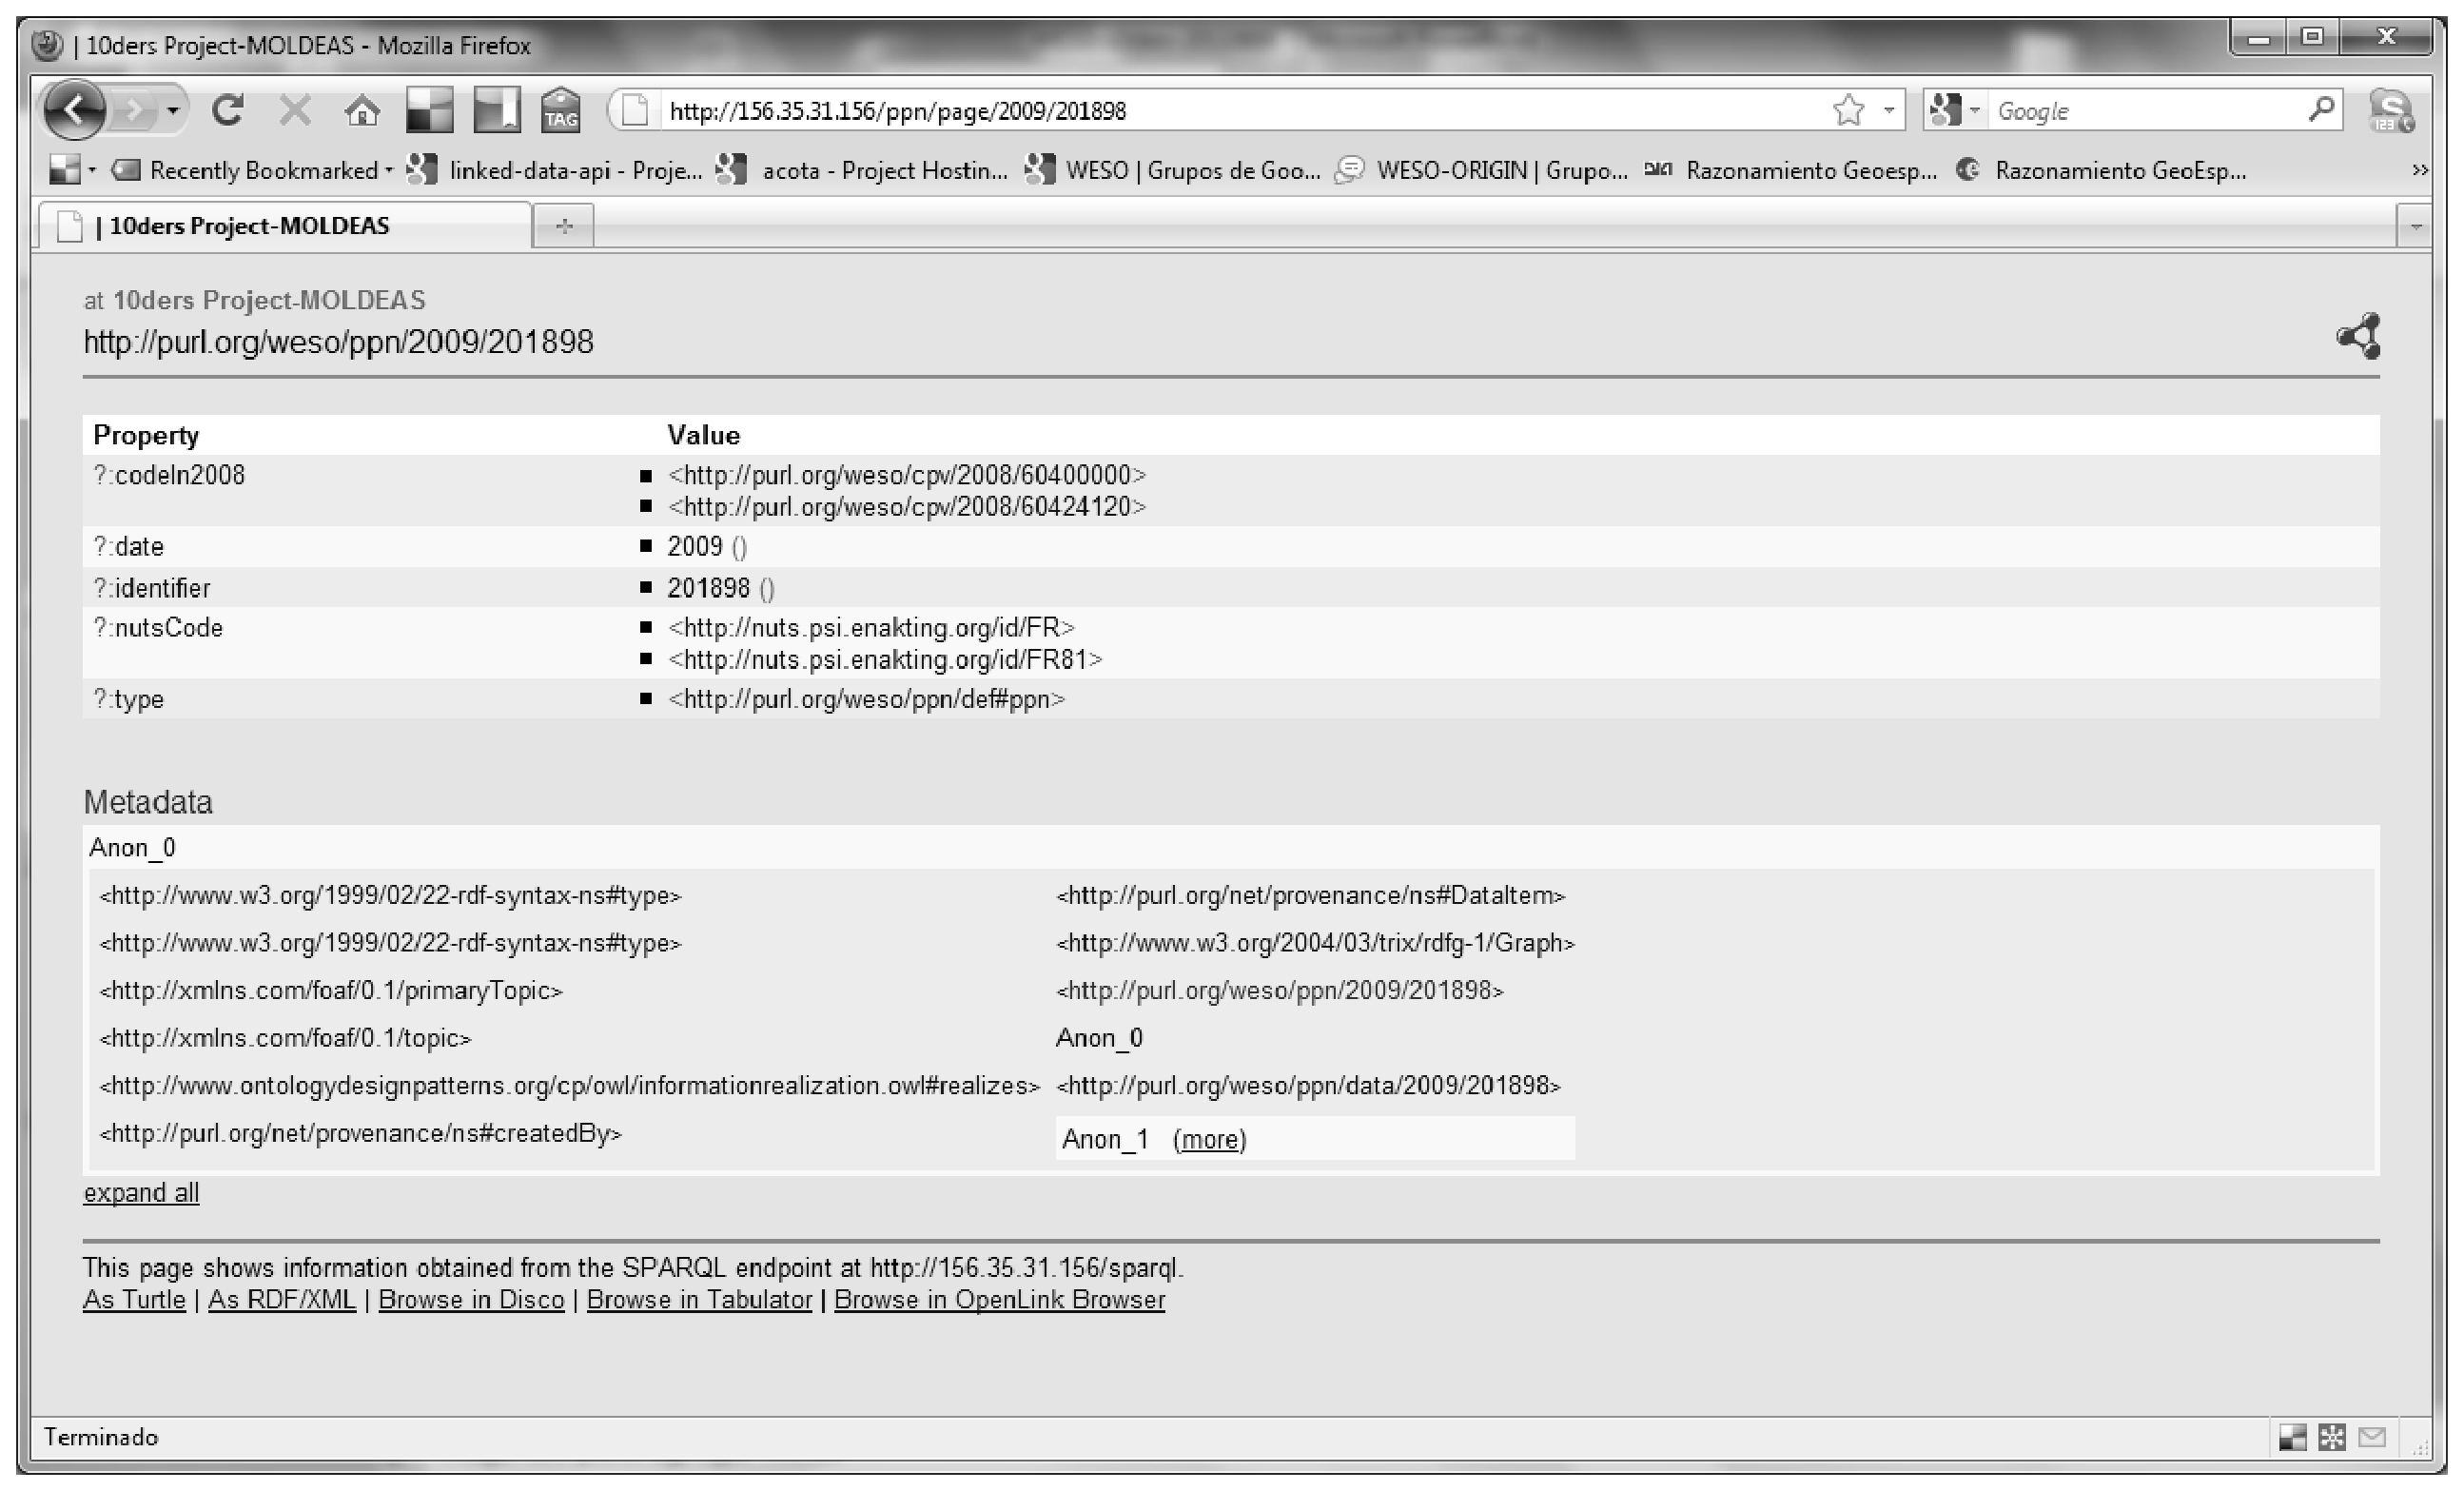
\includegraphics[width=14cm]{images/phd/moldeas/moldeas-pubby}
\caption{Acceso a los datos enlazados mediante Pubby.}
\label{fig:moldeas-pubby-screen}
\end{figure}


\item Finalmente y con el objetivo de ejemplificar el uso de \gls{SPARQL} y las posibilidades 
de consultas al \texttt{endpoint} se han creado una serie de consultas representativas 
para que los usuarios más técnicos tengan la posibilidad de configurar y crear sus propias 
consultas, ejecutándolas y obteniendo los resultados directamente. Para suministrar esta funcionalidad 
se ha utilizado la herramienta \gls{SNORQL}, ver Figura~\ref{fig:moldeas-snorql-screen}.

\begin{figure}[!htb]
\centering
	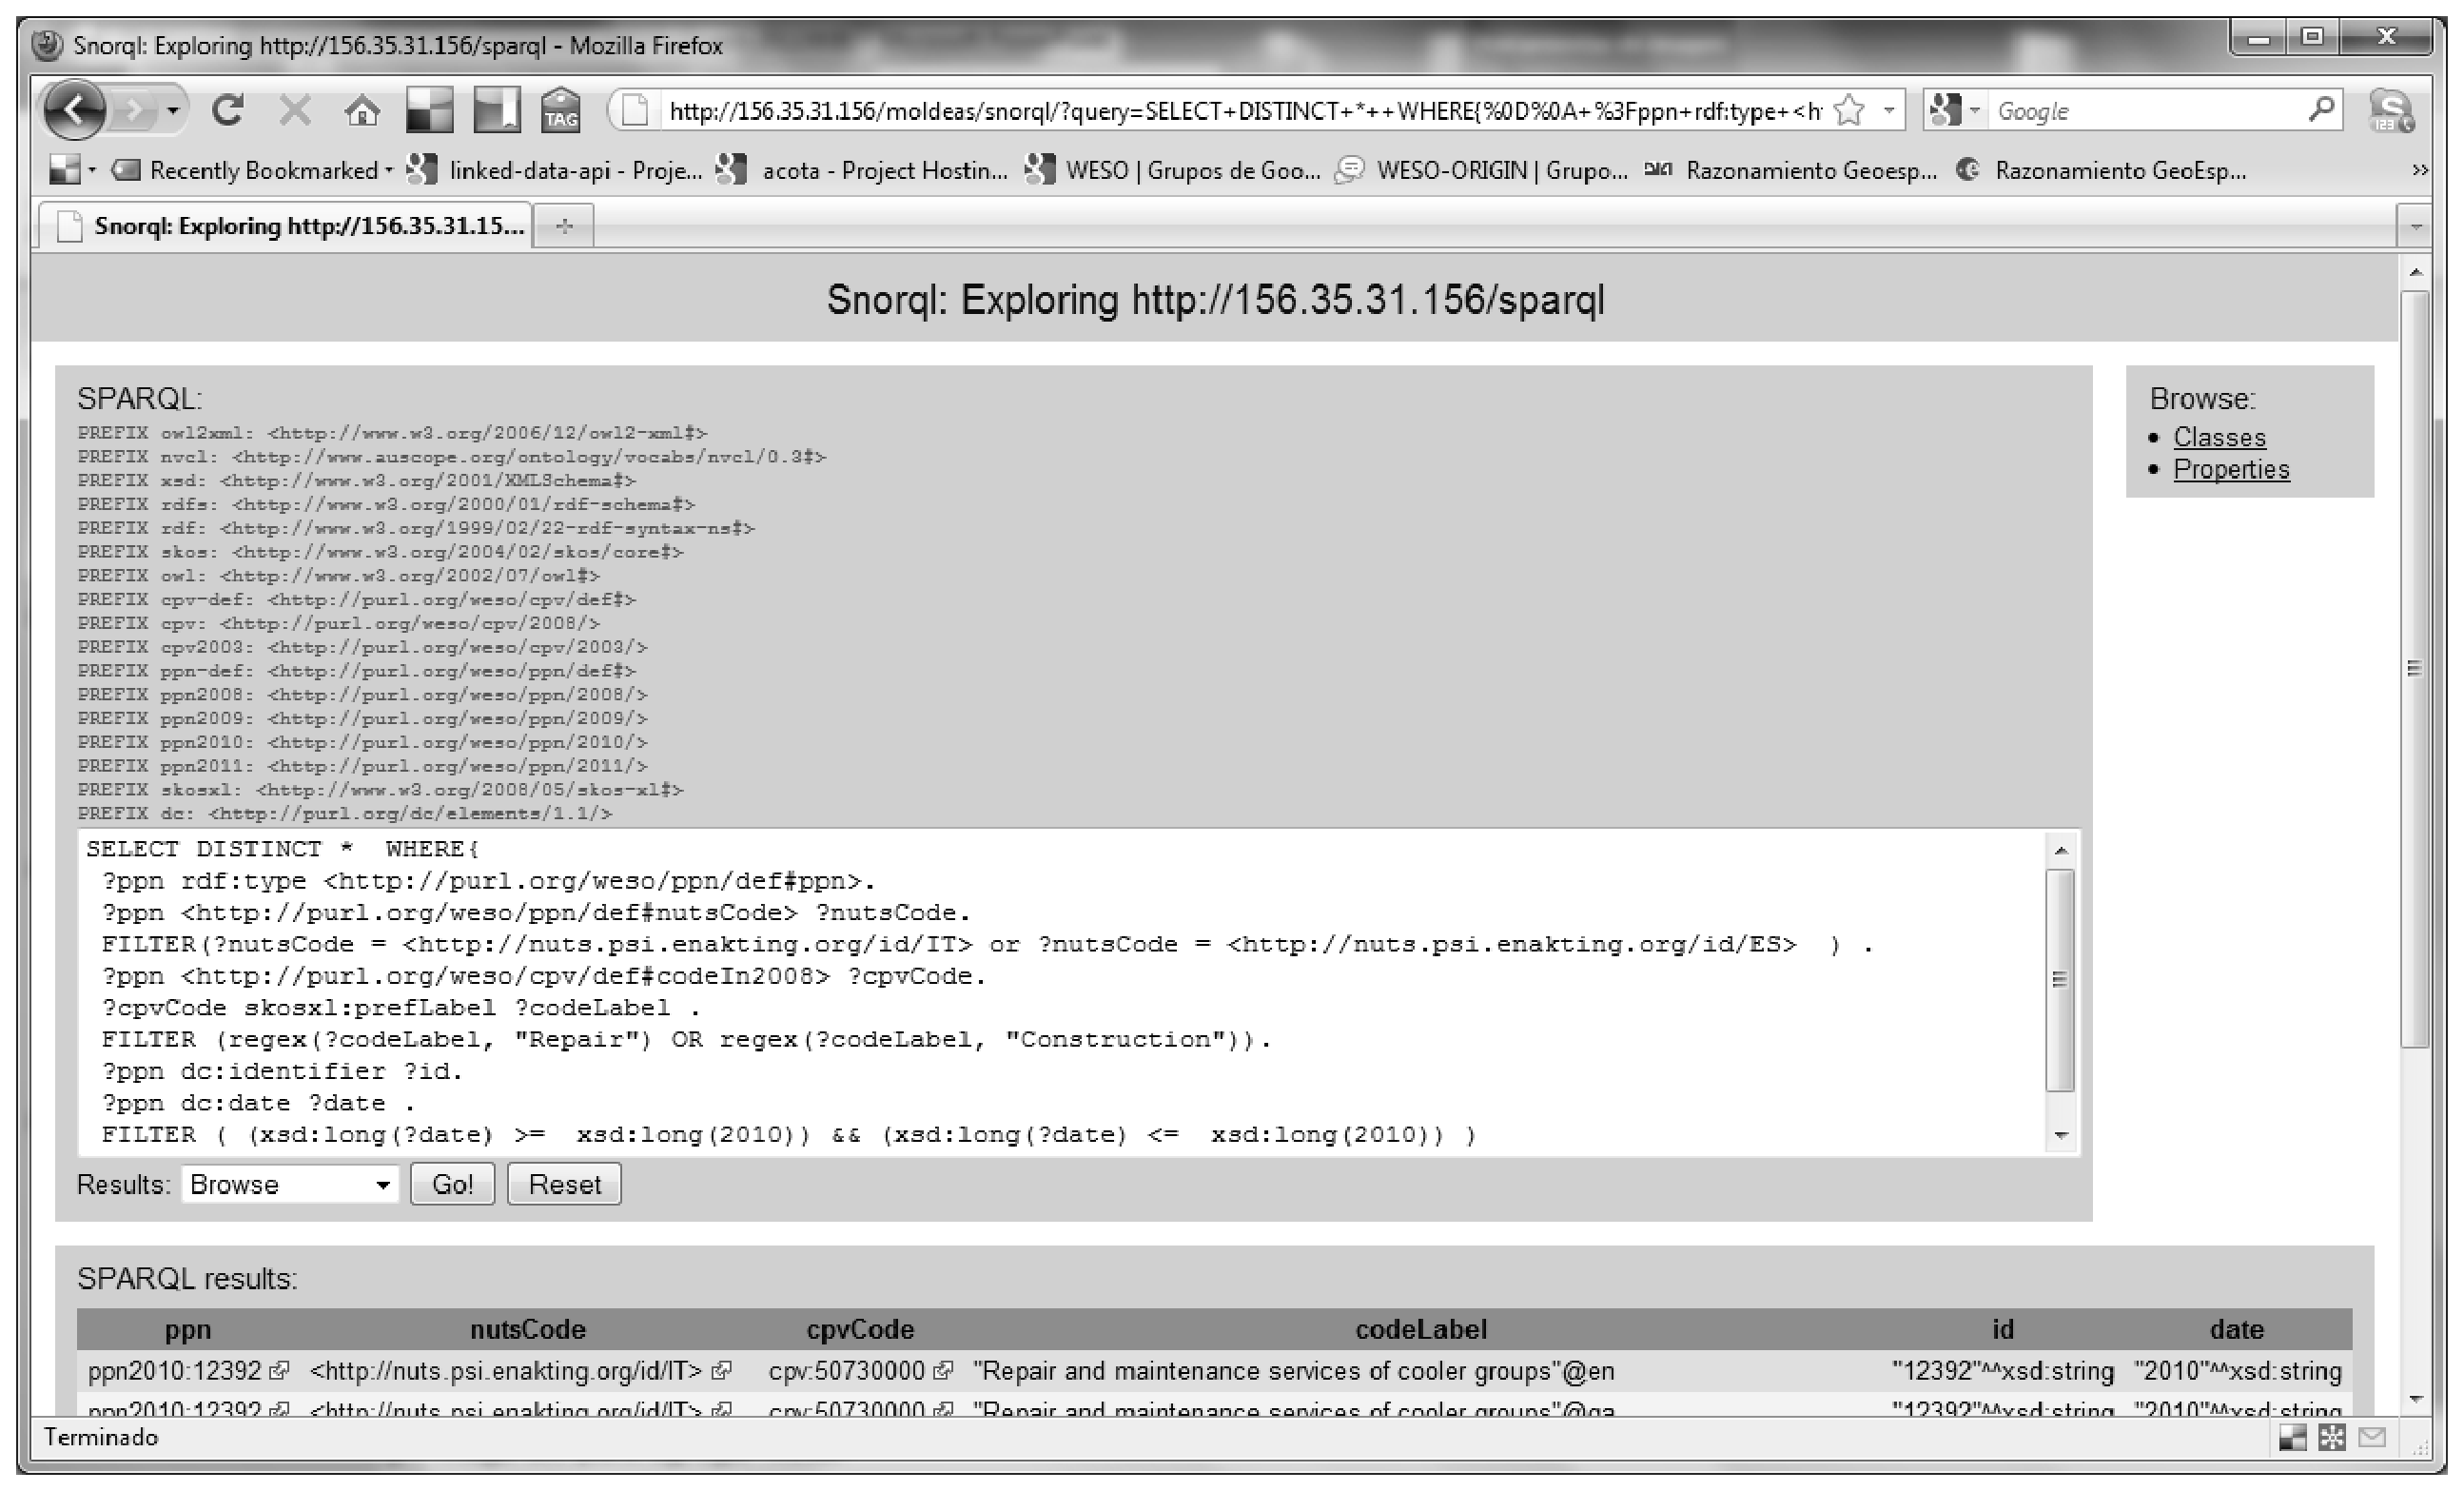
\includegraphics[width=14cm]{images/phd/moldeas/moldeas-snorql}
\caption{Consulta a los datos enlazados mediante SNORQL.}
\label{fig:moldeas-snorql-screen}
\end{figure}



\end{enumerate}







